\documentclass{iau}
\usepackage{graphicx,natbib,url}
\bibliographystyle{apj}
 
\newcommand{\apj}{ApJ}           % Astrophysical Journal
\newcommand{\apjl}{ApJ}           % Astrophysical Journal
\newcommand{\mnras}{MNRAS}       % Monthly Notices of the RAS
\newcommand{\nat}{Nature}
\newcommand{\aap}{A\&A}
\newcommand{\aaps}{A\&AS}
\newcommand{\araa}{ARA\&A}
\newcommand{\aj}{AJ}
\newcommand{\pasp}{PASP}
\newcommand{\apjs}{ApJS}           % Astrophysical Journal
\newcommand{\aapr}{A\&A Rev.}
\newcommand{\na}{New Astr.}

\title{The Stellar Mass of M31 seen by the Andromeda Optical \& Infrared Disk Survey}

\author[Sick et al]{Jonathan Sick,$^1$  Stephane Courteau,$^1$ Jean-Charles Cuillandre,$^2$ Julianne Dalcanton,$^3$ Roelof de Jong,$^4$ Michael McDonald,$^5$ Dana Simard,$^1$ \and R. Brent Tully$^6$}

\affiliation{$^1$Department of Physics, Engineering Physics \& Astronomy, Queen's University, Kingston, ON, Canada K7L 3N6. email: {\tt jsick@astro.queensu.ca}, {\tt courteau@astro.queensu.ca}\\
$^2$CEA IRFU\\
$^3$Department of Astronomy, University of Washington, Box 351580, Seattle, WA 98195, USA. {\tt jd@astro.washingston.edu}\\
$^4$Leibniz Institut für Astrophysik Potsdam (AIP), An der Sternwarte 16, 14482 Potsdam, Germany. {\tt rdejong@aip.de}\\
$^6$Kavli Institute for Astrophysics and Space Research, MIT, Cambridge, MA, USA. {\tt mcdonald@space.mit.edu}\\
$^6$Institute for Astronomy, University of Hawaii, 2680 Woodlawn Drive, Honolulu, HI, USA. {\tt tully@ifa.hawaii.edu}}

\pubyear{2014}
\volume{311}
\jname{Galaxy Masses as Constraints of Formation Models}
\editors{M. Cappellari \& S. Courteau, eds.}

% Figure template
% \begin{figure}
% \centering
% \includegraphics[width=0.5\columnwidth]{cappellari_fig1.eps} 
% \caption{Lorem ipsum dolor sit amet, consectetur adipiscing elit. Duis vel erat eget orci auctor vestibulum fermentum at nibh. Sed eget tempor velit, ac mattis tortor. Integer eget tincidunt dolor. Pellentesque et dui vitae arcu vehicula blandit quis scelerisque velit. Maecenas ultricies lacus ac nibh dapibus tincidunt. Aenean consequat faucibus magna, at malesuada arcu scelerisque vitae.}\label{fig:fig1}
% \end{figure}

\begin{document}

\maketitle

\begin{abstract}
Our proximity and external vantage point make M31 an ideal testbed for understanding the structure of spiral galaxies.
The Andromeda Optical and Infrared Disk Survey (ANDROIDS) has now mapped M31's bulge and disk out to R=40 kpc in ugriJK bands with CFHT using a careful sky calibration programme.
Here we present Bayesian modelling of the optical-infrared spectral energy distribution to yield profiles of M31's stellar populations and mass along the major axis.
This analysis provides evidence for inside-out disk formation and a declining metallicity gradient.
M31's $i$-band mass-to-light ratio ($M/L_i^*$) decreases from 0.5~dex in the bulge to $\sim 0.2$~dex at 40~kpc.
The best-constrained models are made against the full $ugriJK_s$ SED, and are also consistent with optical-only SED fits.
Thus NIR data can be successfully modelled with modern stellar population synthesis, though NIR data do not appear to provide significant extra constraints in this application.
Fits to the $gi$-SED alone yield $M/L_i^*$ that are systematically lower by 0.1~dex.
Relations of $M/L_i$ via $g-i$ colour found in the literature systematically differ by 0.3~dex, reminding us of the importance of stellar population priors and modelization in estimating accurate stellar masses.
We advocate a stellar mass of $M_*(30~\mathrm{kpc})=10.3^{+2.3}_{-1.7}~\mathrm{M}_\odot$.
\keywords{galaxies: elliptical and lenticular, cD - galaxies: evolution - galaxies: formation}
\end{abstract}

\firstsection
\section{Introduction}

We conceived of ANDROIDS to be a homogeneously-calibrated map of M31's bulge and disk in $ugriJK_s$ bands with CFHT MegaCam and WIRCam to enable global studies of M31's structure and stellar populations.
In this contribution, we use ANDROIDS to estimate the stellar mass profile of the M31 disk within $R_\mathrm{maj}\sim40$~kpc using optical and NIR SED measures.


\section{M31 Surface Brightness Calibration}

Background subtraction is the most significant systematic uncertainty in the ANDROID's map of M31, and dramatically affects our ability probe the stellar populations of M31's outer disk.
This is particularly accute in the our NIR maps where skyglow is 3-dex brighter than the disk, while also have strong spatial and temporal variations.
In \cite{Sick:2014} we described the ANDROIDS/WIRCam sky-target nodding and background subtraction schemes.
In summary, we found that the NIR background cannot be known to better than 2\% given the scale of sky-target nods required for M31.
We can overcome this uncertainty by asserting that each overlapping pair of images in our mosaics should have consistent surface brightness and proceed to solve for sky offsets for each frame that formally minimize these surface brightness differences.
Such sky offsets are on the order of 1\% of the NIR brightness.
While the mosaics are smooth up the level of residual background \emph{shape} uncertainties, the zeropoint normalization of NIR sky offsets is significant---up to 0.16\% of the sky level.
In optical bands, the sky background is both more stable and far less bright, though we still employ sky-target nodding with the Elixir-LSB method for CFHT/MegaCam to build a real-time map of sky and scattered light backgrounds over one-hour sliding windows.
With Elixir-LSB we easily identify low surface brightness features in M31's outer disk, such as the Norther Spur, at levels below $\mu_g~26$~mag~arcsec$^{-2}$.

The aforementioned sky offset zeropoint uncertainty requires that are profiles, through particularly at NIR, be finely calibrated against external datasets.
Resolved stellar catalogs transfomed into surface brightness maps, such as our own WIRCam star catalog, but even Panchromatic Hubble Andromeda Treasury (PHAT) provide a useful dataset up to the limit of completeness corrections.
Our WIRCam star catalog profile, in particular, allows us to correct and extend our NIR SB profiles beyond $R_\mathrm{maj}=40$~kpc (though our SED measurements shown here are resicted to just the estent our of pixel maps).
Extremely wide-field imaging is also useful since background can be sampled simultaneously with the disk light.
We are currently using Dragonfly (CITE) to image M31 and replace the wide-field Schmidt telescope plates of \cite{Walterbos:1987}.

\section{SED Stellar Mass Modelling}

\begin{figure}
\centering
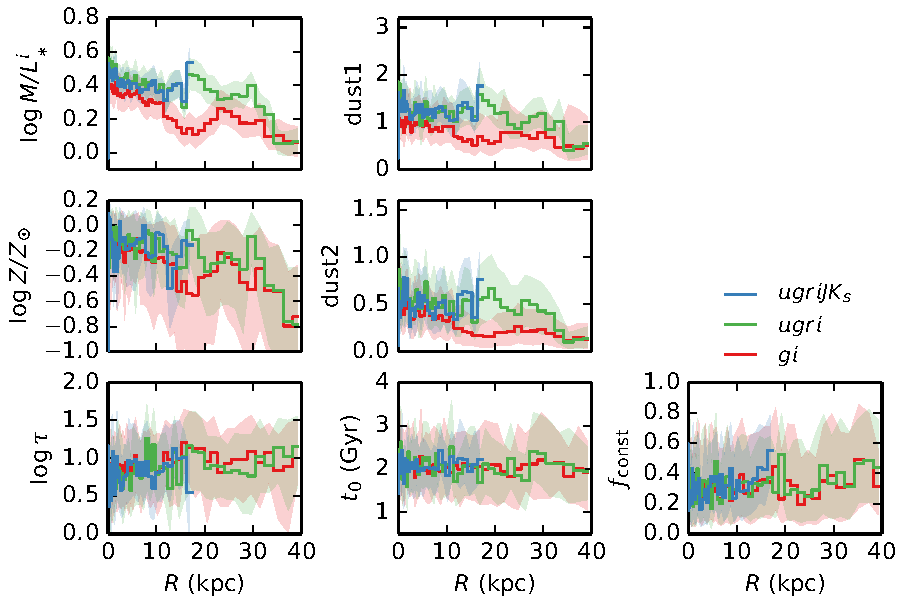
\includegraphics[width=0.5\columnwidth]{pop_profile} 
\caption{Posterior stellar population profiles.}\label{fig:pop_profile}
\end{figure}

\begin{figure}
\centering
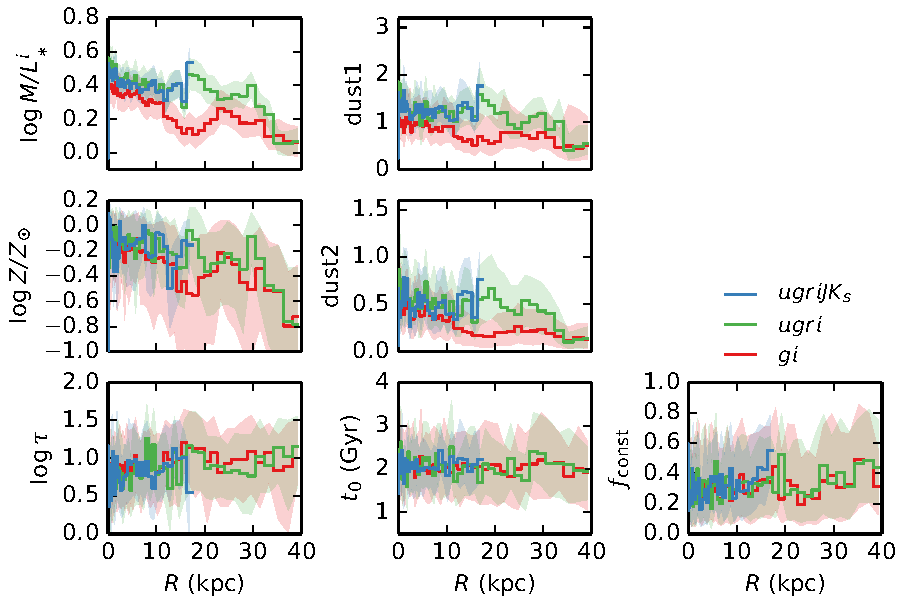
\includegraphics[width=0.5\columnwidth]{pop_profile} 
\caption{Posterior stellar $M/L_i^*$ (left) and mass (right) profiles.}\label{fig:mass_profile}
\end{figure}

From the calibrated surface brightness profiles, we model the SED at each radial bin to estimate the stellar population, and hence the stellar mass-to-light ratio, $M/L_i^*$.
Our modelling engine is the Flexible Stellar Population Synthesis (FSPS) software\footnote{\url{http://people.ucsc.edu/~conroy/FSPS.html}} \citep{Conroy:2009,Conroy:2010}.
We chose FSPS both because it is well-calibrated and known to have a `lighter' AGB contribution than older SP models \citep[e.g.,][]{Bruzual:2003} and also because it's application programming interface allows deep customization of the computed stellar populations.
One author (J.S.) contributes to the maintenance of a Python-language wrapper for FSPS.\footnote{\url{http://dan.iel.fm/python-fsps}}.

We use a Bayesian method to model each SED extracted along the northern major axis of the M31 disk.
Unlike some authors at this Symposium who marginalize over libraries of pre-computed stellar populations, we use a Markov Chain Monte Carlo approach to explore the stellar population distributions of each SED.
This MCMC is nearly trivial to implement with the emcee\footnote{\url{http://dan.iel.fm/emcee}} python package \citep{Foreman-Mackey:2010} that uses an affine-invariant sampler \cite{Goodman:2009} to automatically tune the step sizes through parameter space (a detail which otherwise plagues the simpler Metropolis-Hastings sampler).

Given its flexible nature, we briefly explored which stellar population and dust parameterizations minimized along with which ensembles of bandpasses produced the most robust stellar population estimates.
Briefly, we found that a simple `$\tau$' model, involving constant plus exponentially declining star formation rate components minimized residuals compared to more sophisticated `delayed $\tau$' and late burst models.
Of the dust attenuation treatments, the default power-law attenuation law with separate components for young and older stellar populations also minimized residuals compared to Milky Way or starburst attenuation models.

Perhaps most interesting was the realization that SED residuals are minimized by fitting the entire $ugriJK_s$ SED.
This runs contrary to previous advice from \cite{Taylor:2011} and \cite{Zibetti:2009} who advocated ignoring NIR bands in mass estimation due to uncertain AGB treatments in the previous generation of stellar population synthesis models \citep[e.g.][]{Bruzual:2003,Maraston:2005}.
Besides the near-infrared, the $u$-band is also crucial: the $griJK_s$-fit SED had has little predictive power over the $u$-band as the optical fit had over the NIR.
This result should encourage SED modellers to incorporate as many bandpasses as possible, including UV and IR, to obtain the best constraints on stellar populations and masses.

Armed with our favoured stellar population parameterization, we modelled SEDs extracted from a logarithmically-sized wedge \citep[e.g.][their Fig. 2]{Courteau:2011} to produce stellar population profiles (shown in Fig. \ref{fig:pop_profile}).
Our posterior profiles, show the basic features of a radially declining metallicity gradient and inside-out disk formation.
More tightly constrained profiles could be obtained through both informative priors and modelling SEDs resolved in the 2D plane.

Perhaps most surprising, though, is that the $ugri$-fit and $ugriJK_s$-fit SEDs produce statistically identical stellar population profiles, with the only exception being a slightly tighter posterior credible region from the full-SED fits
Although the consistency of optical and optical-NIR SED fits is reassuring from the perspective of near-infrared calibrations, it is also disappointing that the NIR data has not produced a remarkably improved posterior stellar population estimate.
Certainly this result is anecdotal, and could change with different underlying stellar populations and dust distributions.

What is clear, though, is that poorly sampled SEDs can bias results.
Fitting only the $gi$ SED (that is, using an input information equivalent to those using colour-M/L look-up-tables) clearly biases the posterior stellar population distribution, with significantly lower dust opacities and lower mass-to-light ratios. 
By comparison, we have also plotted mass-to-light ratios predicted by three colour-M/L fits \citep{Zibetti:2009,Taylor:2011,Into:2013}.
These fits systematically vary by 0.3~dex, far larger than the 0.1~dex of internal systematic uncertainty typically claimed by $g-i$ -- $M/L$ fits. 
Compared to our full SED fits, modelling of the $gi$ SED is less biased than these other M/L fits, which are based on other stellar population synthesis models.
This serves as reminder that stellar mass estimates remain dominated by prior assumptions such as choices of IMF, dust, and details of AGB treatments, among other concerns.

Given this discussion, we estimate a stellar mass of the M31 disk, within $30$~kpc, as $M_{ugri}^{*} = 10.3^{+2.3}_{-1.7}~\mathrm{M}_\odot$.
This result is consistent with the stellar bulge and disk masses quoted by \cite{Tamm:2012} (10.1~$\mathrm{M}_\odot$).

\section{Discussion}

We are currently using these stellar mass maps in concert with dynamical tracers of gas and stars to construct a mass model of M31's stellar, gas, and dark matter components.
\cite{Tamm:2012} recently constructed a mass model of M31 using dynamical tracers along with SDSS and Spitzer 3.6~$\mu$m photometry.
Their bulge models are ill-constrained due to a lack of dynamical tracers within 8~kpc.
However, we use the DiskFit code (CITE) to correct for non-circular motions in HI kinematics in \cite{Saglia:2010} and {Chemin:2010} measurements that reach the centre of M31.
The success of this mass model will be determined by the stability of a dynamical N-body realization with the GalactICS code (CITE).


\section*{Acknowledgements}

\noindent TODO

% \begin{thebibliography}{99}

% \bibitem[{{Bruzual} \& {Charlot}(2003)}]{bruzual03}
% {Bruzual} G., {Charlot} S., 2003, \mnras, 344, 1000

% \end{thebibliography}

\bibliography{master}

\end{document}
